\documentclass{article}
\author{Jonathan Dyer}
\title{CS 1699: Privacy in the Electronic Society \\
        \textit{Project 2 -- Access Control Policies}}

\usepackage{amsmath}
\usepackage{amsthm}
\usepackage{enumitem}
\usepackage[margin=0.8in]{geometry}
\usepackage{graphicx}
\usepackage[backend=bibtex,type=alphabetical,sorting=ynt]{biblatex}
\addbibresource{p2.bib}

% ============ USED FOR MY FORMAT ============
\providecommand{\task}[1]{\section{Task #1}}
\providecommand{\soln}{\textbf{Solution: }}
\providecommand{\image}[1]{
    \begin{center}
        \includegraphics[width=1.0\textwidth]
            {#1}
    \end{center}
}
\providecommand{\tightlist}{
    \setlength{\itemsep}{1pt}\setlength{\parskip}{0pt}
}
\providecommand{\inlinecode}{\texttt}
\providecommand{\RT}{\textbf{RT}}

% ============ USED FOR CODE LISTINGS ============
\usepackage{listings}
\usepackage[usenames,dvipsnames,svgnames]{xcolor}
\definecolor{javagreen}{rgb}{0.25,0.5,0.35}
\lstdefinelanguage{XML}
{
  basicstyle=\ttfamily\footnotesize,
  morestring=[b]",
  moredelim=[s][\bfseries\color{Maroon}]{<}{\ },
  moredelim=[s][\bfseries\color{Maroon}]{</}{>},
  moredelim=[l][\bfseries\color{Maroon}]{/>},
  moredelim=[l][\bfseries\color{Maroon}]{>},
  morecomment=[s]{<?}{?>},
  morecomment=[s]{<!--}{-->},
  commentstyle=\color{DarkOliveGreen},
  stringstyle=\color{blue},
  identifierstyle=\color{red}
}

\lstset{
  frame               = single,
  language            = XML,
  numbers             = left,
  showstringspaces    = false,
  keywordstyle        = \color{blue},
  mathescape
}

\setcounter{secnumdepth}{0} % sections are level 1


\begin{document}
\maketitle

\bigskip

\tableofcontents

\bigskip

\task{W0}
\subsection{$\RT_0$: Role-based Trust management with attributes}
The access-control language selected for this project is a simplified variant of a family of expressive languages known as $\RT$, which is short for \textit{\textbf{R}ole-based \textbf{T}rust-management}.
In spite of the name, the $\RT$ family is actually an extension of role-based access control (RBAC) known as \textit{attribute}-based access control (ABAC).
It fulfills all of the desirable traits mentioned in \cite{RTmain}, including delegation of attribute authority, inference of attributes, and more.
By allowing explicit subject abstraction and specific attribute assignment to those subjects, the system provides the same functionality that roles do via selection by attributes and intersection of attributes along with even greater flexibility and expressiveness.
The language utilized here is based on a combination of $\RT_0$ and $\RT_2$, and functions as follows: \\
\begin{itemize}
  \item The primary structures in this framework are \textit{entities} (or principals), \textit{subjects} (or users), \textit{roles} (which contain rights or permissions), and \textit{objects} (or resources).
  \item \textbf{Entities} are simply the organizations or systems that issue credentials (i.e. assign roles to users). By explicitly abstracting entities, the $\RT$ framework allows for localized roles, as well as more extensive delegation.
  \item \textbf{Subjects} are the users or agents in the system. They may have one or more roles that provide them with permissions (or authorized actions) for accessing objects in the specified way.
  \item \textbf{Roles} are a convenient way of grouping permissions that may be assigned to subjects. Roles may be hierarchical--if a role dominates another, then it has every permission the other role has. This helps reduce the number of roles and relationships that have to be dealt with in the system. Role assignment may be achieved by specifying subject attributes.
  \item \textbf{Objects} are the elements whose access is being controlled by this entire schema. They may be grouped by attribute as well, allowing flexible and powerful specification of permissions.
  \item Each structure accepts descriptive \textit{attributes} that enable powerful specification of policies based on any desired combination of subject, role, or object attributes. This, in conjunction with the outline above, facilitates the following features (among others): \\
  \begin{enumerate}
    \item \textbf{Indirection}: Because we can specify policies according to attributes, we may assign i) a set of permissions (i.e. a role or multiple roles), to ii) a set of users, over iii) a set of objects, as long as those sets can be well-defined or uniquely specified (i.e. all elements in the desired set must share an attribute that specifies exactly that set).
    \item \textbf{Delegation}: Different entities that assign roles (within their domain) may easily defer to the authority of another entity for checking role membership. That is to say, if organization $A$ defines role $r_1$, it is simple to write a policy that includes into $r_1$ all members of role $r_2$ from some other organization $B$ as well. This is also referred to as 'delegation of attribute authority', meaning that if $B$ says that some subject has attribute $r_2$, then $A$ says it has attribute $r_1$ (here speaking of roles as attributes of users). Details of how this is done are given in the next section.
    \item \textbf{Role Hierarchy}: Roles may inherit permissions from other roles given by the same entity. This is a variant of delegation, in a sense allowing an organization to delegate authority over some role attribute to that same organization under another role attribute. Thus, role management is simplified and duplication is reduced.
    \item \textbf{Logical Objects}: Inspired by $\RT_2$, the current variation of this framework also supports collections of objects, known as Object Groups, which allows addition by attribute and assignment of permissions respecting objects \textit{en masse}. In other words, it is possible to define a role with an access mode and an entire group of logically-related objects (via attributes) rather than just one object at a time.
    \item \textbf{Attribute Intersection}: Support of multiple attributes on any given element in the system also allows specification of policies by intersection of attributes. For instance, it is possible to specify an action that is allowed only for users who are in the intersection of multiple roles (i.e. users that have each of those roles).
  \end{enumerate}
\end{itemize}
It is important to note that there are many other extensions and variations in the $\RT$ language family, and the current iteration was chosen as a convenient balance between expressiveness and feasibility for the purposes of the current project. Many other features are possible within the $\RT$ framework, such as parameterization of attributes, threshold policies, and more. \par
Further, it is important to note that the original specification of $\RT$ also included details regarding the issue of \textit{common vocabularies} across entities. This issue of vocabularies or namespaces is dealt with via \textit{application domain specification documents (ADSDs)}, but was ommitted here for brevity's sake, and because it is not relevant to the ideas being explored. For more information however, and generally for a great amount of detail regarding the $\RT$ family of languages, see \cite{RTmain} and \cite{RTold}.


\task{W1}
\subsection{Overview of Syntax and Policy File Format}
The syntax chosen to write policy files for the above language is straightforward and designed for maximal ease and clarity. It is encoded in XML, and comprises two primary sections in every entity for which policies are being defined: 1) Data, and 2) Policies. \par
\textbf{Data} is where all elements of the entity are specified, and includes the following:
\begin{itemize}\tightlist
  \item A full definition of any objects in the entity, including object groups and any attributes associated with them.
  \item A definition of all roles and their corresponding permissions, including all objects/object groups those roles affect and any role hierarchy that exists natively (independent of any particular policy).
  \item Specification of all subjects or users given credentials (i.e. assigned roles) in the entity, with all relevant attributes included.
\end{itemize}
\textbf{Policies} is the section where any of the extra features or relationships are defined. Although some of the basic access policies are implicitly encoded in the Data section, more advanced relationships are expressed here, including:
\begin{itemize}\tightlist
  \item Delegation of authority.
  \item Assignment of permissions using logical objects (i.e. objects grouped by attribute).
  \item Access that relies on attribute intersection.
  \item Any attribute inference or other complex relationships.
\end{itemize}

Thus an overall outline of the policy file may look like this: \\
\begin{lstlisting}
<?xml version="1.0"?>
<!-- The <root> element simply contains everything and exists for parsing convenience -->
<root>
    <entity name="Entity 1">
        <data>
            <objects>
              ...       <!-- All object groups and resources go here -->
            </objects>
            <roles>
              ...       <!-- All role groups and permissions go here -->
            </roles>
            <subects>
              ...       <!-- All subjects and their attributes go here -->
            </subjects>
        </data>
        <policies>
          ...           <!-- All specific policies go here -->
        </policies>
    </entity>

    <entity name="Entity 2">
      ...               <!-- Repeat for as many entities as you're defining -->
    </entity>
</root>
\end{lstlisting}

In keeping with generally accepted XML style, all core and necessary features of an element are contained in sub-elements, while optional or incidental data, including tags (or attributes) are contained as XML attributes in the opening tag. \par

It is important to note that the description here is for a basic outline of a policy file, including implementation of features 1-5 above. Further extensions and options are possible and may be made available at a later time, but this describes the minimum syntax necessary to write an access control policy file with these features in \RT using an XML encoding.

\subsubsection{Entities}
The only thing to know about the \inlinecode{<entity>} element is that it has a single attribute called 'name' by which you may indicate the name of the entity. \par

Otherwise, each section necessary for an entity's fully-described policy is explained forthwith.

\subsection{Data}
The \inlinecode{<data>} tag has no attributes, so we will move directly into considering objects, roles, and subjects.
\subsubsection{Objects}
This section is straightforward, and the easiest to define.
The \inlinecode{<objects>} tag itself takes no attributes, but rather serves to enclose the section. Two types of elements can be contained in this section:
\begin{enumerate}\tightlist
  \item Object groups, denoted by the \inlinecode{<objectGroup>} tag, must have a name and otherwise may take any attributes desired.
  \item Individual objects, denoted by the \inlinecode{<object>} tag, must have a name and otherwise may take any attributes desired. They may also have a group specified as a sub-element \inlinecode{<group>}.
\end{enumerate}

Our first feature is introduced in this section, namely feature 4: \textit{Logical Objects}. This refers to the ability to specify objects in one of 3 ways: 1) individually by name, 2) as a collection via a formalized Object Group such as 'Files' or 'Printers', or 3) as a collection by any identifying attribute that specifies the desired objects uniquely.
Here I give an example of method (1)--specifying objects individually--and show how method (2) is represented, but give full details of Logical Objects (including (2) and (3)) later on in section \textbf{W5}.




\subsubsection{Roles}
Filler.

\subsubsection{Subjects}
Filler.


\subsection{Policies}
Filler.
\subsubsection{Inference}
Filler.
\subsubsection{Delegation}
Filler.
\subsubsection{Logical Objects}
Filler.



\task{W3}
Explain with 2 examples how to implement \textit{indirection}.

\task{W4}
Explain with 2 examples how to implement \textit{delegation}.


\task{W5}
Explain with examples how to implement \textit{2 other features}.


\pagebreak

\section{Task W7}
\subsection{Algorithm B: Constant-Time Comparison}
Now let's examine \textbf{Algorithm B} so that we can understand how and why this revised algorithm runs in a more constant-time manner, mitigating some of the effects discussed for Algorithm A above.
In the pseudocode below, first notice that before anything else we select a consistent number of iterations to run the byte-wise comparisons for (\inlinecode{len} in the code below, line 5)--this helps ensure that we don't reveal information about the length of the secret value (perhaps a login name), since that was an obvious and large timing difference in our naive algorithm.
Next, consider the revised loop through our inputs (lines 9-13). Rather than breaking this loop once we find a mismatch, we continue for the specified length \inlinecode{len} (line 9).
Then we check that both of the next characters are even valid to be compared (line 10). If so, we skip to the \inlinecode{else} (line 12) and proceed with the comparison. If either one is \textit{not} valid, we execute a "dummy" comparison to (hopefully) take the same amount of time as a real one (line 11).
Finally, we return the resulting boolean.

\begin{lstlisting}
// This method takes two strings, a and b, and returns True if they are equal, False otherwise
def algorithm_B (String a, String b)

  // We'll assume string a is the "system string" we're comparing the user-input against
  int len = a.length

  // Now set a boolean and then iterate through characters, comparing each (even on mismatch)
  boolean bool = (a.length == b.length)
  for i in $0 \dots$ len                  // for every character in the fixed length
    if a[i] == null || b[i] == null       // if we've reached the end of one string
      bool = (a[0] == a[0]) && bool       // compare something anyways
    else                                  // otherwise
      bool = (a[i] == b[i]) && bool       // compare the two chars, update the boolean

  return bool
\end{lstlisting}


\subsection{Results}
Benchmarking the above code -- implemented in Ruby -- over 1000s of iterations gives the results displayed in the table below. Note that the timing distinctions between the different types of comparison are almost entirely eliminated for shorter strings, and are statistically insignificant for longer strings/hash values. It is worth noting that comparing strings of different length still seems to be notably faster, especially for shorter inputs. This could reveal the length of a secret, given enough samples.

\image{constant_results.png}

The improvement is especially clear given the graph below, which shows much more even timing results across different types of input. In particular, the test on longer (hash) strings shows a slight reversal in the trend across strings of the same length--which could indicate that it would lead an attacker to make incorrect guesses (a desirabe trait).

\image{constant_graph.png}

\subsection{Trade-Offs \& Design Decisions}
There is a significant performance cost associated with making constant-time comparisons, especially when trying to obscure even the length of the secret value(s). Notice in the comparison graph below for Naive vs. Constant Comparison that the constant-time algorithm takes nearly twice as long when comparing similar strings and \textit{several times} as long when comparing very different strings. This would be a highly significant cost on a system or web-server that may receive thousands of requests a day/hour/minute. \par

\begin{center}
    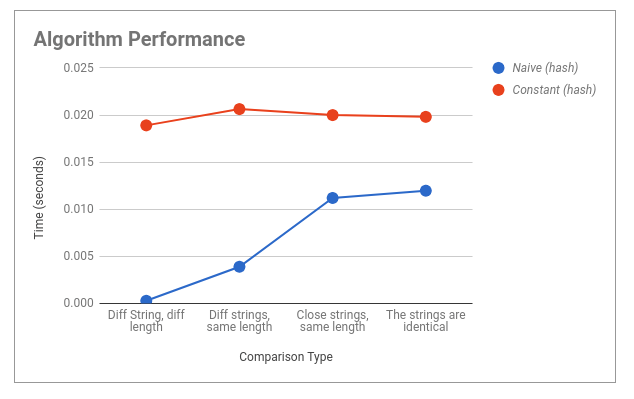
\includegraphics[width=0.8\textwidth]
        {alg_perf.png}
\end{center}



\pagebreak

\printbibliography[heading=bibintoc]

\end{document}
